\section{The Testbench Architecture}

Compared to the development process of the previous introductory step, the adoption of the \uvm allowed me to move past the low-level intricacies of setting up the testbench environment with all the components and utilities I could need, and focus instead on a smaller set of \dut-specific problems; most notably:
\begin{itemize}
    \item Interfacing the \dut and the environment through the agent
    \item Crafting the reference model to validate the \dut responses to the random stimulus
    \item Devising the functional coverage model to measure progress
    \item Configuring the reporting system to easily post-process the results of the simulation runs
\end{itemize}
This resulted in faster and higher quality development, as I was taking advantage of an already extensively tested code base and I could direct the saved time and efforts toward the most challenging problems of the designs I had to verify. The conceptual representation of the testbenches is shown in~\cref{fig:duts_tb}, with the detailed interface for the windowed register file in~\cref{fig:wrf_if}

Each testbench project can be partitioned into three core components:
\begin{enumerate}
    \item A \sv interface to bundle the \dut wires. It simplifies both connectivity, as it can be instantiated like a module and connected to ports like a signal, and synchronization, through clocking blocks that encapsulate the timing specifications of signals that are read or driven by the testbench synchronously to a clock.

    \item A \sv package to collect the verification classes and utilities, similar to the \svinline{uvm_pkg}. This simplifies source management, given that all the definitions and declarations pertaining to a testbench are available in a package ready to be imported into the top module.

    \item A top-level module and program block. The program block ensures race-free interaction between the design and the testbench at the simulation kernel level and has the fundamental job of starting the execution of the \uvm test; it is instantiated taking as input the interface, which is shared through virtual handles in the configuration database to the monitors and drivers.

    The top module contains the instances of the \dut, the interface, and the program block. In addition, it hosts the clock generator, that I chose to implement here, being it more closely tied to the design domain rather than to the testbench. 
\end{enumerate}

\subsection{Reusability}
A key idea to reusability is to separate structure from behavior. Being transactions, or specifically sequence items, the main communication vehicle across the boundary, their modeling has paramount importance and should come early in the development flow.
Moreover, to maximize code reuse and further decrease the bug rate, I strived to take advantage of inheritance to avoid code duplication between the two projects.

\subsubsection{Sequence Item Design}
In both \dut namespaces I defined:
\begin{description}
    \item[\svinline{class RqstTxn}] Having chosen to adopt the sequence mechanism, the request transaction is defined to extend \svinline{uvm_sequence_item} and has two main purposes:
    \begin{itemize}
        \item It's created through the factory by sequences and randomized to generate the stream of sequence items to feed the driver. Its data members are the ones the driver translates to pin wiggles onto the signals in its modport and are qualified to undergo randomization. 
        
        I avoided adding randomization constraints in this class, with the idea that tests can use the factory and override this type with a child class that includes test and stimulus-specific constraints; specifically, \svinline{CnstRqstTxn}. The advantage is that in case simulation runs had highlighted coverage holes, I would've been able to add tests with different constraints to target the remaining cases.

        \item It serves as the parent for the response transaction class. Given that the scoreboard needs to compare the expected and actual \dut responses, to add robustness I implemented the method \svinline{do_compare()}, called internally by \svinline{compare()}, to preliminary assess whether the responses pertain to the same request or not.
    \end{itemize}
    Notice that to improve simulation performance I always print transaction objects through the \uvm report functions passing the string generated by \svinline{convert2string()}. The alternative would be to implement \svinline{do_print()} and invoke \svinline{print()}, but it introduces a significant overhead.
    
    \item[\svinline{class RspTxn}] It's the transaction used in analysis communication, broadcasted by the monitor, outside the agent and to subscriber components in the environment. It encapsulates the data members worth capturing with the monitor: the request fields are inherited by extending \svinline{RqstTxn} and having both the request and response fields available in the broadcasted transactions is crucial for scoreboard operation. This is because I chose to embed the reference model that processes requests and generates expected responses within the scoreboard.

    This approach has a downside that became evident when tackling the windowed register file: when request-response pairs are collected in an overlapping fashion, if it's possible for the current request to abort the previously sampled one, whose response is currently being sampled, a mechanism to inform the scoreboard is needed. As a consequence, for the windowed register file, \svinline{RqstTxn} is extended by \svinline{RqstAnlysTxn}, which adds a field to mark the request as aborted, and the latter is then extended by \svinline{RspTxn}.
\end{description}


\subsubsection{Shared Base Classes}
Although agents share a common structure for stimulus generation and response capturing, the \uvm library already ships the necessary abstractions for its implementation and the number of base classes to be manually developed and shared between projects is minimal. 
 
First, it's good practice to avoid directly using the \svinline{uvm_sequencer} class and define an extended class registered with the factory that will be displayed when printing the testbench topology; this is done with \svinline{class Sequencer}.
For the components outside of the agent, in addition to the base coverage collector class described in~\cref{subsec:func_cov}, there are:
\begin{description} 
    \item[\svinline{class Printer}] The printer listens on the analysis port and prints the incoming transactions both to the screen and to a file log. 
    The key aspects of file logging are that the printer retrieves the file path from the configuration database in the build phase; then, in the end-of-elaboration phase, it associates the id \svinline{"printer"} to the printer file descriptor and to the action \svinline{UVM_DISPLAY | UVM_LOG}. On the contrary, \svinline{class BitBucket} extends \svinline{Printer} and sets as action \svinline{UVM_LOG}, to only print transactions to the log file.

    If debugging messages are enabled, by raising the verbosity at least to \svinline{UVM_HIGH}, the printer reports a state dump in case of a successful configuration.
    
    \item[\svinline{virtual class BaseScoreboard}] It's the abstract base class that implements those anticipated common duties of scoreboards as response checkers, but are the child classes the ones that implement the pure virtual function \svinline{generate_prediction()} based on a reference model. Like a printer, it listens on the analysis port to incoming transactions: 
    \begin{itemize}
        \item in the \svinline{write()} callback function, it clones the incoming \dut response for its request fields and generates the expected response. If the comparison yields a mismatch, an error is reported both on screen and to the scoreboard log file; otherwise, the match is only logged to file. 

        The only difference in the file logging management from the printer is that, in the end-of-elaboration phase, the id \svinline{"scoreboard"} is associated with different actions depending on the severity, so that only mismatch reports with severity \svinline{UVM_ERROR} reach the screen.

        \item if the job of stopping the simulation was entirely left to sequences, which drop objections as soon as the driver notifies \svinline{item_done()} on the last sequence item, the \dut wouldn't be able to respond in time and, consequently, also the monitor and its subscribers. The solution I implemented is the following. In the build phase, \svinline{BaseScoreboard} clears a flag that only gets set once the number of expected responses matches the ones actually received. In the phase ready-to-end, a process is forked to keep an objection raised until the flag gets set.
    \end{itemize}  
    
    \item[\svinline{class Environment}] The two main customization mechanisms of \uvm are the factory and the configuration database. The former allows to change at instantiation time the type of an object being created with a derived one; the latter allows a parent in the testbench topology to define properties for its children. Given that the build phase is called top-down, the parent can't directly set those properties in its build phase, as the layers below don't exist yet; instead, it leaves them packed in a configuration object in the database, so that children can retrieve it when it's their turn to be built.

    The environment is fundamental for both. In its build phase, it retrieves a configuration object of type \svinline{env_cfg_t} from the database: most of the properties within it are put back in the database and passed down the hierarchy. Also, it instantiates the verification components through the factory, thus taking into account overrides requested by the test: for instance, \svinline{Printer} overridden by \svinline{BitBucket}, or \svinline{Coverage} by \svinline{StmCoverage}. Moreover, it takes care of connecting the analysis communication paths.
    
    \item[\svinline{virtual class BaseTest}] According to the common approach presented in~\cref{subsubsec:uvm_arch}, this class takes care of duties common to all tests. Specifically, it configures the environment in a way that is suitable to most tests, leaving the callback \svinline{configure_env()} for them to perform additional tweaking. Considering that I wouldn't have needed tests to coordinate the execution of sequences on multiple agents, I avoided implementing a virtual sequence. Instead, the \svinline{BaseTest} instantiates a \svinline{TopSequence} object through the factory: this way, not only can I specify a different \svinline{TopSequence} class in each project namespace, but tests can also override it through the factory if needed.
    
    Another fundamental job is to take care of processing command line plusargs:
    \begin{itemize}
        \item The file paths for the printer and scoreboard logs
        \item The flag \verb|+quiet| to enable the \svinline{BitBucket} override
        \item \verb|+n_txn| to choose the number of request transactions per test sequence to generate
    \end{itemize}

    Also notice that when the verbosity is at least \svinline{UVM_HIGH}, for debugging purposes it prints the topology of the hierarchy, the content of the configuration database and a summary of the state of the factory.
\end{description}

\subsection{Intel's Pentium IV Adder}\label{subsec:p4-adder}

\begin{sidewaysfigure}
    \thisfloatpagestyle{empty}
    \centering
    \subfloat[][Intel's Pentium IV Adder.\label{fig:p4_adder_tb}]
        {\raisebox{1.25cm}{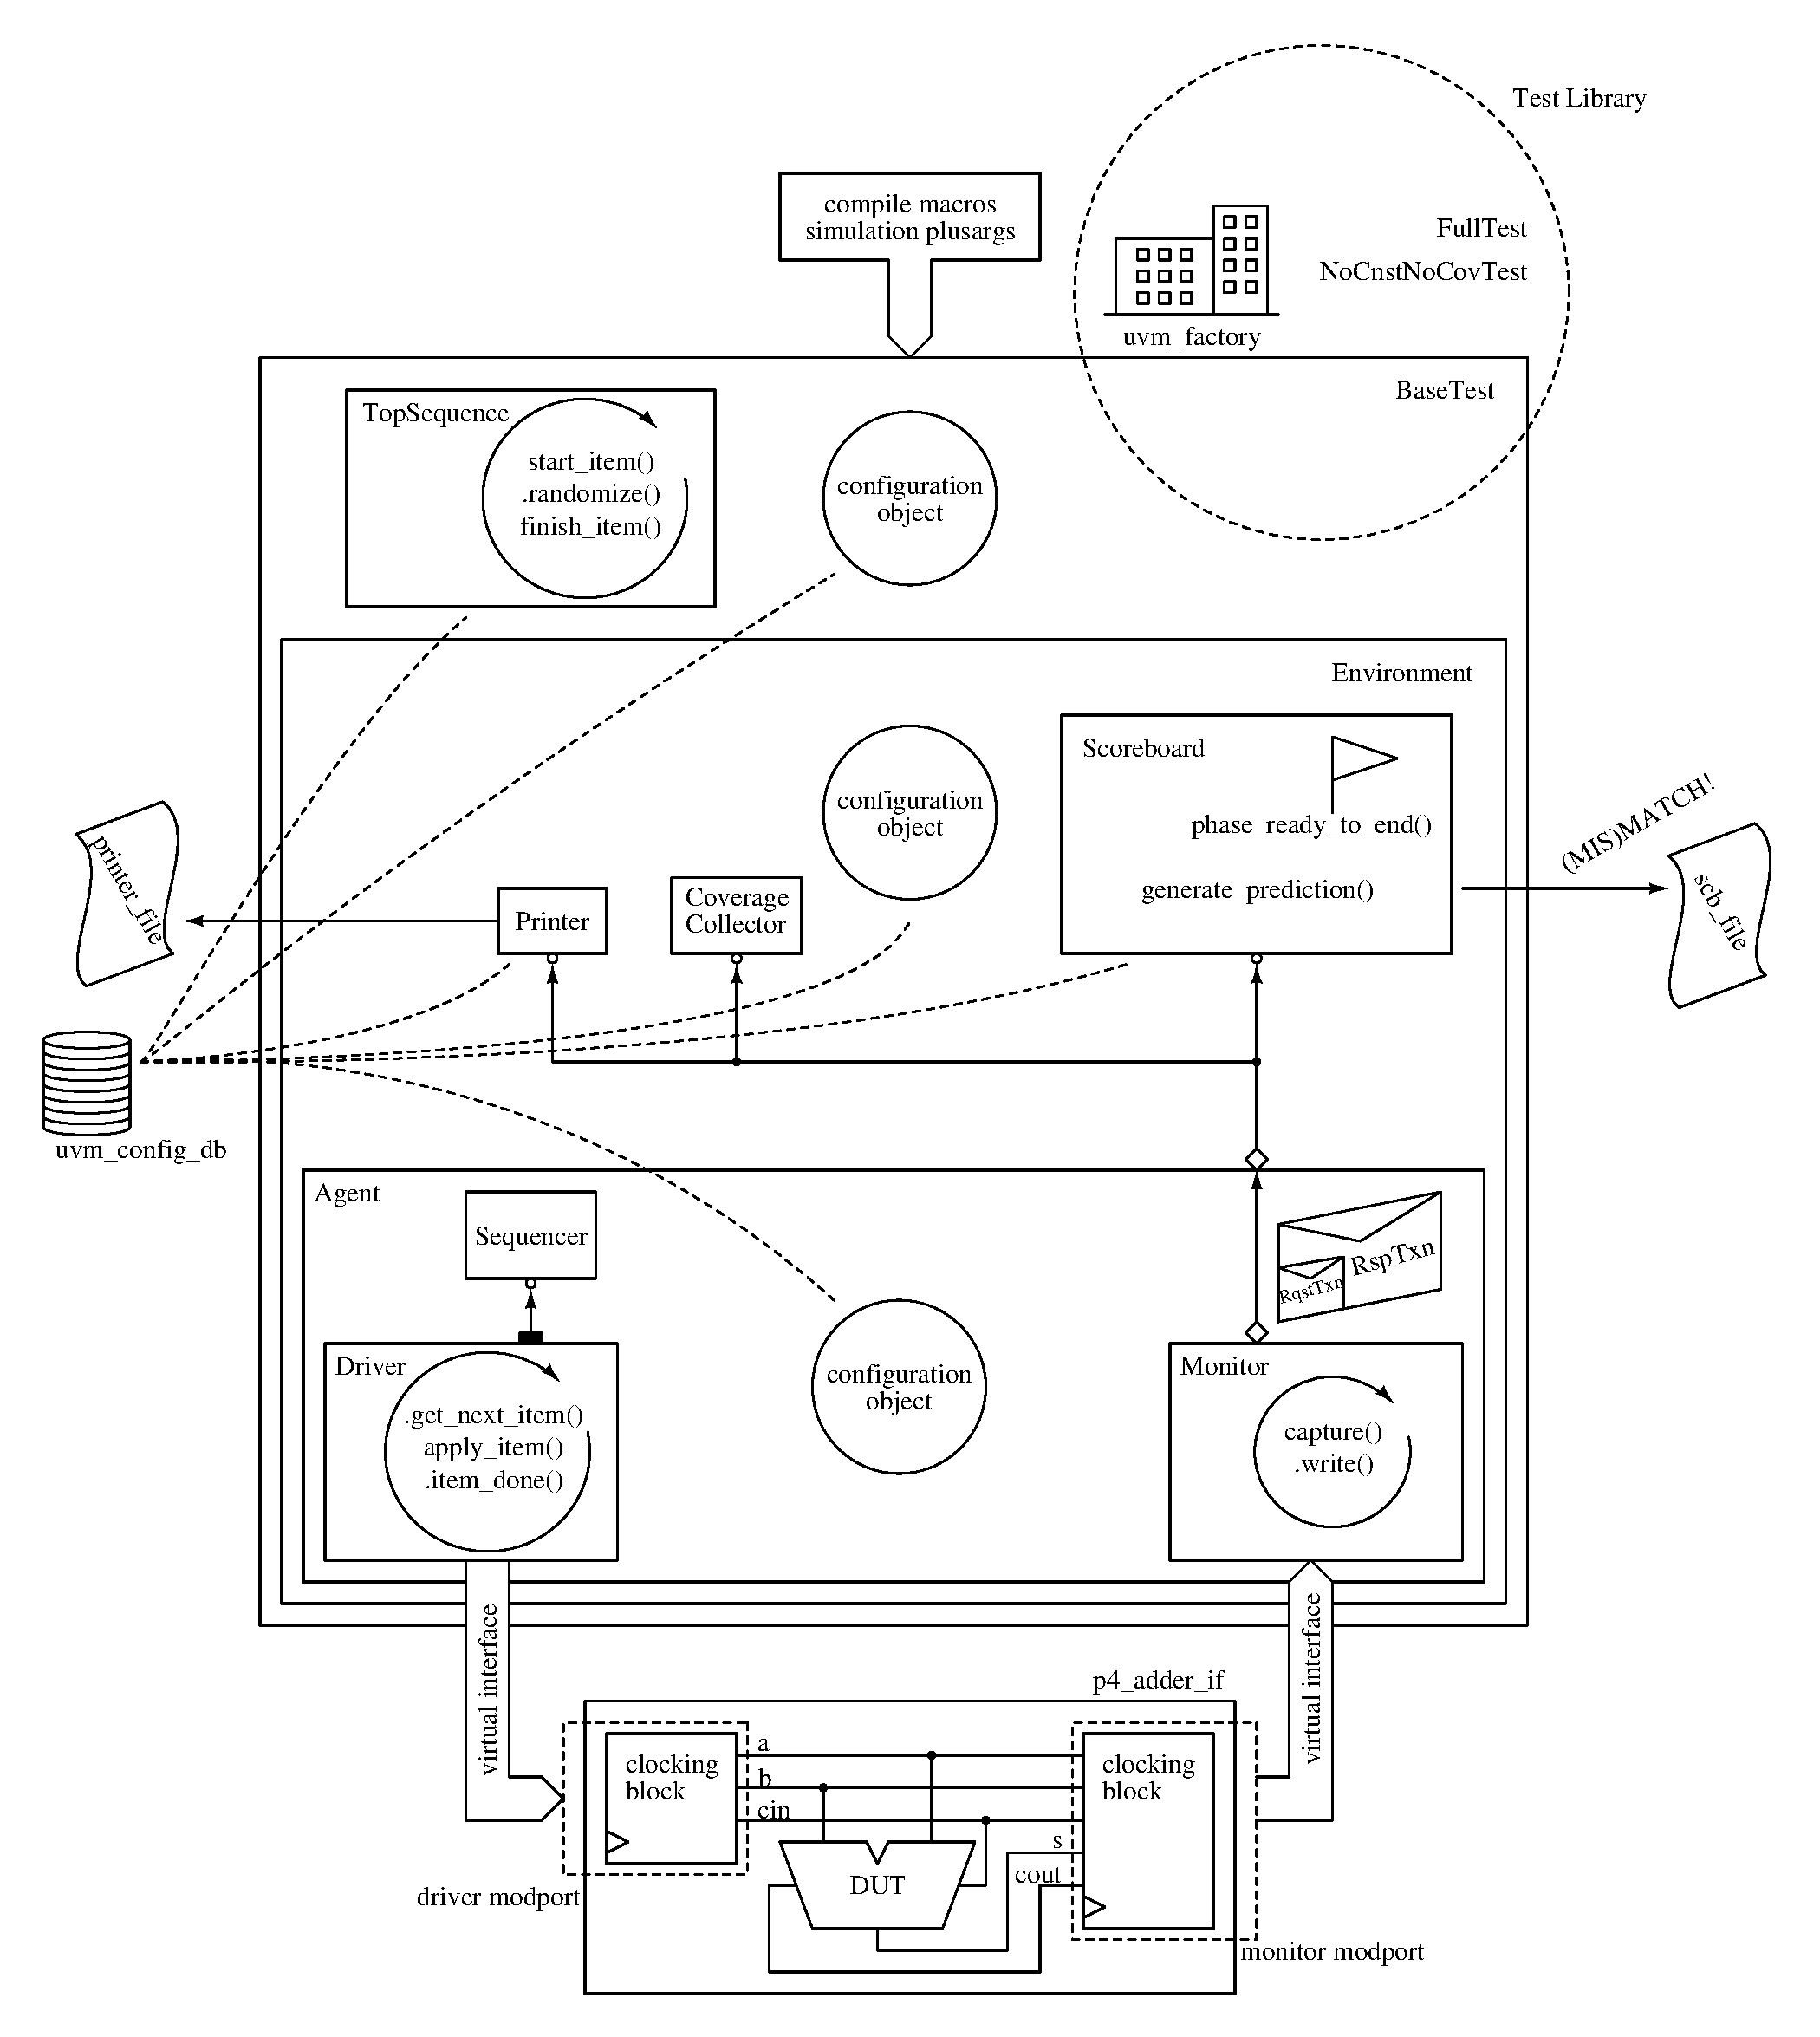
\includegraphics[width=.48\linewidth]{fig/p4_adder/p4_adder_tb_architecture.eps}}}\qquad
    \subfloat[][Fixed-Size Windowed Register File.\\In red, the main differences compared to the adder testbench.\label{fig:wrf_tb}]
        {\includegraphics[width=.45\textwidth]{fig/windowed_rf/windowed_rf_tb_architecture.eps}}
    \caption{Conceptual representation of the \acs{uvm}-based testbenches and their connection to the {\acs{dut}}s.}
    \label{fig:duts_tb}
\end{sidewaysfigure}

\begin{listing}
\begin{minted}[bgcolor=backcolor, fontsize=\scriptsize]{systemverilog}
constraint ab_dist_c {
  a dist { // skew a towards the boundaries
    0                       := 1,
    [1 : {NBIT{1'b1}} - 1]  :/ 1, // spread
    {NBIT{1'b1}}            := 1
  };
  b dist {
    0                       := 1,
    [1 : {NBIT{1'b1}} - 1]  :/ 1, // spread
    {NBIT{1'b1}}            := 1
  };
};
\end{minted}
\caption{Weighted distribution constraint for the input operands of Intel's Pentium IV adder.}
\label{list:p4_cnst}
\end{listing}

\noindent Starting from the interface, \cref{fig:p4_adder_tb} shows that the interaction with the \dut is carried out through the driver and the monitor modports. Given that the circuit is combinational, I chose the following synchronization. The driver drives \svinline{a}, \svinline{b} and \svinline{cin} according to the clocking block defaults, namely \qty{0}{\nano\second} after the rising edge of the clock; then, \svinline{1step} before the subsequent rising edge, not only the monitor can sample the response of the adder, \svinline{s} and \svinline{cout}, but also the driven request, which is still valid.

As for the verification components tailored to the Pentium IV adder, the most interesting aspects are:
\begin{description}
    \item[\svinline{class Agent}] The driver and monitor virtual modport handles are retrieved in the build phase by the agent from its configuration object stored in the database. Only once the entire hierarchy has been built, in the connect phase, the agent can use them to initialize the monitor and driver data members. 

    \item[\svinline{class Scoreboard}] It extends \svinline{BaseScoreboard} to specify the reference model and the implementation of the \svinline{generate_prediction()} callback. Given that the reference model is the addition operator inherent in the language, once having cloned the response transaction for its request fields the prediction boils down to a sum.

    \item[\svinline{class CnstRqstTxn}] It extends \svinline{RqstTxn} to add the constraint in~\cref{list:p4_cnst} and skew the stimulus towards the boundaries of the representation interval, in an attempt to reduce the number of request transactions needed to cover the verification plan.
\end{description}

Making use of the techniques described earlier, two extended tests are available:
\begin{description}
    \item[\svinline{class NoCnstNoCovTest}] It's used to debug the active part of the testbench early in the development stages. It instantiates the environment as configured by \svinline{BaseTest}: the generated request transactions are fully unconstrained and there is no coverage collector.
    \item[\svinline{class FullTest}] It overrides \svinline{RqstTxn} with \svinline{CnstRqstTxn} and configures the environment to instantiate a coverage collector, overridden with \svinline{StmCoverage}.
\end{description}

\subsection{Fixed-Size Windowed Register File}\label{subsec:wrf}

\begin{figure}
    \centering
    \includegraphics[width=.7\linewidth]{fig/windowed_rf/windowed_rf_if_schematic.eps}
    \caption{Detailed representation of the interface with the fixed-size windowed register file. The memory management unit has a dedicated modport through which it can respond to spill and fill requests: it samples the \vhdlinline{reset} signal; during the spill operation it samples the \vhdlinline{spill} and \vhdlinline{out1} and drives \vhdlinline{mmu_done}; during the fill operation it samples \vhdlinline{fill} and drives both \vhdlinline{mmu_data} and \vhdlinline{mmu_done}.}
    \label{fig:wrf_if}
\end{figure}

\begin{listing}
\begin{minted}[bgcolor=backcolor, fontsize=\scriptsize]{systemverilog}
task apply_item(input RqstTxn rqst);

  /* synchronize on the driving active edge */
  @(vif.drv_cb);

  /* rf busy spilling/filling */
  if (!rqst.reset && vif.bypass) begin
    uvm_report_info("debug", "rf bypassed: waiting", UVM_HIGH);

    @(negedge vif.bypass);
    uvm_report_info("debug", "rf bypassed: fell", UVM_HIGH);

    @(vif.drv_cb);
  end

  vif.drv_cb.reset   <= rqst.reset;
  ...
  
endtask : apply_item
\end{minted}
\caption{Snippet of the driver logic to translate incoming sequence items to signal-level. When the windowed register file is busy with a spill or fill operation, the translation is temporarily halted until the falling edge of the \svinline{bypass} signal notifies the end of the operation. Only a reset request is allowed to pass through during this time.}
\label{list:wrf_drv}
\end{listing}


\begin{listing}
\begin{minted}[bgcolor=backcolor, fontsize=\scriptsize, escapeinside=||]{systemverilog}
  task run_phase(uvm_phase phase);
    RspTxn rqst1, rqst2;

    /* skip init */
    @(vif.mon_cb);

    forever begin
      /* first edge */
      capture(|\tikzmark{dLeft}|rqst2|\tikzmark{dRight}|, |\tikzmark{aLeft}|rqst1|\tikzmark{aRight}|); // rsp to rqst2, rqst1
      if (rqst2 != null) begin
        ap.write(rqst2);
        uvm_report_info("capture", {"first edge: ", rqst2.convert2string()}, UVM_HIGH);
      end

      /* second edge */
      capture(|\tikzmark{bLeft}|rqst1|\tikzmark{bRight}|, |\tikzmark{cLeft}|rqst2|\tikzmark{cRight}|); // rsp to rqst1, rqst2
      if (rqst1 != null) begin
        ap.write(rqst1);
        uvm_report_info("capture", {"second edge: ", rqst1.convert2string()}, UVM_HIGH);
      end
    end
  endtask : run_phase
\end{minted}
\begin{tikzpicture}[remember picture, overlay]
  \DrawArrows[red, out=-120, in=60]{a}{b}
  \renewcommand{\VerticalShiftStartArrows}{0,+.15}%
  \renewcommand{\VerticalShiftEndArrows}{0,-.05}%
  \DrawArrows[blue, in=-60, out=120]{c}{d}
\end{tikzpicture}
\caption{Snippet of the monitor logic designed to manage the overlapped sampling on the rising edges of both the current request, which was driven on the preceding falling edge of the clock, and the pending response, whose request had been already sampled on the prior rising edge. The red arrow emphasizes that a request sampled on a rising edge is advanced to collect its response on the subsequent rising edge. The blue arrow underscores the same event, offset by one clock cycle.}
\label{list:wrf_mon}
\end{listing}

\begin{listing}
\begin{minted}[bgcolor=backcolor, fontsize=\scriptsize]{systemverilog}
class Mmu extends uvm_component;

  /* behavioral stack in main memory */
  data_t mem[$];

  task run_phase(uvm_phase phase);

    /* fsm thread handler */
    process fsm_th;

    forever begin
      fork // separate fsm and synchronous reset

      begin : fsm_p

        fsm_th = process::self();

        forever begin
          @(vif.mmu_cb);

          if (vif.mmu_cb.spill) begin
            /* do spill */
          end

          else if (vif.mmu_cb.fill) begin
            /* do fill */
          end
        end
      end : fsm_p

      /* in case of a reset, restart the machine */
      begin : synch_reset_p

        do
          @(vif.mmu_cb);
        while (!vif.mmu_cb.reset);

      end : synch_reset_p

      join_any // the synchronous reset thread

      fsm_th.kill();
      fsm_th = null;
      mem.delete();
    end
  endtask : run_phase

endclass
\end{minted}
\caption{Skeleton implementation of the memory management unit. In the run phase task, two processes are spawned: one containing the actual logic to respond to fill and spill requests, based on the signals sampled on the rising edges of the clock; the other is an alarm process devised to detect synchronous resets, kill the \acs{fsm}, clear the stack in main memory and respawn both processes.}
\label{list:wrf_mmu}
\end{listing}

\begin{listing}
\begin{minted}[bgcolor=backcolor, fontsize=\scriptsize]{systemverilog}
class CnstRqstTxn extends RqstTxn;

  /* call/return balancing:
   * count how many returns are possible */
  int unsigned can_return;
  byte unsigned ret_weight;

  function void post_randomize();

    /* balance */
    if (reset)
      can_return = 0;
    else begin // could be both call and ret, but call wins
      can_return += call;
      can_return -= (ret && !call);
    end
  endfunction : post_randomize

  constraint valid_ret_c {
    ret  dist {
      0 := (100-ret_weight),
      1 := (can_return ? ret_weight : 0)
    };
  }

endclass
\end{minted}
\caption{Snippet of the adjustment of the distribution weight for the random bit \svinline{ret} to guarantee the validity of return requests. When the unsigned counter \svinline{can_return} reaches 0, the \svinline{ret} bit is restricted from assuming the value 1 until a subsequent successful call request occurs.}
\label{list:wrf_cnst}
\end{listing}

\noindent Comparing the testbench architectures in~\cref{fig:duts_tb}, the first difference is in the interaction with the \dut. The windowed register file acts as a circular-buffer implementation for the top of the stack maintained in the main memory, thus I developed a verification component that emulates the memory management unit, intending for it to be instantiated within the driver. The interface is detailed in~\cref{fig:wrf_if}. The driver communicates with the \dut through two separate modports:
\begin{itemize}
    \item The driver modport is the one used to translate the incoming sequence items to signal-level. All \dut input signals, except \svinline{mmu_data} and \svinline{mmu_done}, are driven \qty{0}{\nano\second} after the falling edge of the clock, via a clocking block. This is because the windowed register file is active on the rising edge of the clock.

    The modport additionally includes an input for the driver: the \svinline{bypass} signal, which the driver uses to determine whether the windowed register file is currently occupied with a spill or fill operation. When such an operation is ongoing, the driver temporarily halts the translation of incoming sequence items until the register file becomes available again, which happens after the falling edge of the \svinline{bypass} signal. Only a reset request is allowed to pass through during this time, as it can abort the preceding fill or spill request. The \sv details are in~\cref{list:wrf_drv}.

    \item The memory management unit has a dedicated modport, which bundles all the signals needed to respond to spill and fill requests. The inputs to the memory management unit are sampled \svinline{1step} before the rising edge of the clock, whereas the outputs, \svinline{mmu_data} and \svinline{mmu_done}, are driven \qty{0}{\nano\second} after it.
\end{itemize}
The monitor job is more complex due to the sequential nature of the \dut, which typically takes a clock cycle to respond, except when dealing with call requests that initiate a spill operation, in which case the response is delayed by an additional cycle. Both the request and the response are sampled on each rising edge of the clock, but the logic to distinguish between the two is within the monitor and is shown at high-level in~\cref{list:wrf_mon}. In the interface, the monitor modport simply bundles all the \dut signals, both inputs and outputs, synchronizing their sampling on the rising edge of the clock through a clocking block.

As for the remaining verification components, the most interesting aspects are:
\begin{description}
    \item[\svinline{class Mmu}] The memory management unit extends \svinline{uvm_component} and implements the protocol described in~\cref{subsec:handson} to respond to spill and fill requests. Conveniently, the model for the stack in main memory is already available in the language through the \sv queue data structure, which can be accessed as a stack through the \svinline{push_back()} and \svinline{pop_back()} methods. 
    
    To model the \ac{fsm}, I chose a behavioral style similar to a SystemC \verb|SC_THREAD| with a synchronous reset. In the run phase task, two processes are spawned:
    \begin{itemize}
        \item The logic that monitors the \svinline{spill} and \svinline{fill} signals, to detect and service spill and fill requests from the \dut.
        \item An alarm process, which wakes up at every rising edge and terminates when the \svinline{reset} signal is sampled high.
    \end{itemize}
    Given that the type of the parallel block is \svinline{join_any}, as soon as the alarm process terminates, the execution of the run phase task resumes. The survivor process is killed, the queue is cleared, and both processes are respawned. The key ideas are illustrated in~\cref{list:wrf_mmu}.
    
    \item[\svinline{class BehWindowedRf}] Unlike the Pentium IV Adder, to extend \svinline{BaseScoreboard} and implement the \svinline{generate_prediction()} callback, I had to develop a behavioral reference model. Working on the idea of the windowed register file as a circular buffer for the top of the stack in main memory, I decoupled these two aspects:
    \begin{itemize}
        \item The storage is implemented with a fixed-size array for the set of global registers and a \sv queue, accessed as a stack, for the windows. The elements contained in the queue are register subsets, the \svinline{subset_t} type, defined as a fixed-size array of registers that can act as \emph{ins}, \emph{locals}, or \emph{outs}. The starting configuration is a queue containing 3 subsets, \emph{ins} and \emph{locals} of the active set, plus the \emph{ins} of the adjacent set addressed as \emph{outs}. Notice that to locate the current window, is sufficient to store the index of the active subset of \emph{locals}. As a consequence:
        \begin{itemize}
            \item Calling is equivalent to pushing a register set, the \emph{locals} and the \emph{outs} subsets of the newly activated window; thus the \emph{outs} of the previously active windows become the \emph{ins}, as soon as the index of the active \emph{locals} is updated.
            \item Vice versa, returning is equivalent to popping a register set.
        \end{itemize}

        \item The circular management is achieved by storing the numbers of the most recent and oldest windows in the stack, traditionally called the \emph{current} and \emph{saved window pointers}. Counting in modulo the total number of windows, the condition:
        \begin{itemize}
            \item Buffer full, which initiates a spill operation, is detected when a call request makes the pointers become equal.
            \item Buffer empty, which initiates a fill operation, is detected when a return request makes the pointers become equal.
        \end{itemize}
    \end{itemize}
    \item[\svinline{class TopSequence}] Considering the higher complexity of the coverage model implemented in \svinline{StmCoverage}, in comparison to the case of the Pentium IV Adder, I chose to make \svinline{TopSequence} a hierarchical sequence object in an attempt to increase the total functional coverage within the same test. Internally, after executing the \svinline{ResetSequence} to establish the same known state for both the \dut and the reference model, the same parametric test sequence \svinline{TestSequence} is executed thrice, each time with parameters fine-tuned empirically to target different portions of the verification plan.
    
    The template parameters of \svinline{TestSequence} serve to customize the randomization properties of the request transaction, which acts as a blueprint object. Notably, among the various constraints introduced by \svinline{CnstRqstTxn} when extending \svinline{RqstTxn}, the key constraint illustrated in~\cref{list:wrf_cnst} ensures the validity of return requests. This is achieved by leveraging the \svinline{post_randomize()} function to dynamically adjust the distribution weight of the \svinline{ret} random bit. The implementation makes use of the unsigned counter \svinline{can_return}, initialized to 0. Following each randomization, the \svinline{post_randomize()} logic assesses whether the request has resulted in a valid call or return operation. In cases of valid calls, the counter is incremented; otherwise, it's decremented. Once the counter reaches zero, the weight assigned to the value 1 for the \svinline{ret} bit is dropped to 0. This effectively enforces a hard constraint that prevents return requests from being issued until the next call request.
\end{description}